\documentclass[
    language=english,
    doctype=lecture-notes,
    institution=none,
]{../../omnilatex}

\RequirePackage{config/document-settings}
\addbibresource{../../bib/bibliography.bib}

\RequirePackage{amsmath,amssymb}
\RequirePackage{algorithm2e}
\RequirePackage{cancel}
\RequirePackage{enumitem}

\DeclareMathOperator{\diag}{diag}
\DeclareMathOperator{\tr}{tr}
\DeclareMathOperator{\rank}{rank}
\DeclareMathOperator{\argmin}{arg\,min}

\begin{document}

\maketitle

% ============================================================
%  CHAPTER 1
% ============================================================
\chapter{Foundations of Numerical Linear Algebra}

\section*{Learning Objectives}
By the end of this chapter, students will be able to:
\begin{enumerate}[label=\textbf{LO\arabic*.}, leftmargin=3em]
    \item Define condition numbers and analyse their effect on algorithm stability.
    \item Derive the LU factorisation with partial pivoting.
    \item Prove convergence bounds for iterative solvers such as Jacobi and Gauss--Seidel.
    \item Implement sparse matrix operations and compare their performance using \textsc{pgfplots}.
\end{enumerate}

% ------------------------------------------------------------
\section{Motivation and Historical Context}

Numerical linear algebra studies algorithms for solving linear systems,
eigenvalue problems, and least-squares problems. Richardson introduced
iterative methods in 1911.\footnote{L.~F.~Richardson, ``The approximate
arithmetical solution by finite differences of physical problems,''
\emph{Phil.\ Trans.\ Roy.\ Soc.\ London}, vol.~210, pp.~307--357, 1911.}
Turing bounded the growth factor of Gaussian elimination in 1948.\footnote{A.~M.~Turing, ``Rounding-off errors in matrix processes,''
\emph{Quart.\ J.\ Mech.\ Appl.\ Math.}, vol.~1, pp.~287--308, 1948.}

% ------------------------------------------------------------
\section{Matrix Conditioning}

\begin{definition}[Condition Number]\label{def:condition}
For a nonsingular matrix $\mathbf{A} \in \mathbb{R}^{n \times n}$, the
\emph{condition number} with respect to a matrix norm~$\|\cdot\|$ is
\[
    \kappa(\mathbf{A}) = \|\mathbf{A}\| \cdot \|\mathbf{A}^{-1}\|.
\]
For the spectral norm ($2$-norm) this reduces to
$\kappa_2(\mathbf{A}) = \sigma_{\max} / \sigma_{\min}$, the ratio of the
largest to the smallest singular value.
\end{definition}

\begin{theorem}[Condition Number Bound]\label{thm:cond-bound}
Let $\mathbf{A}$ be nonsingular and $\mathbf{b}$ a right-hand side. If
$\mathbf{A}$ is perturbed by $\delta\mathbf{A}$, then
\[
    \frac{\|\delta\mathbf{x}\|}{\|\mathbf{x}\|}
    \;\le\; \kappa(\mathbf{A})
           \cdot \frac{\|\delta\mathbf{A}\|}{\|\mathbf{A}\|}.
\]
\end{theorem}

\begin{proof}[Proof of \autoref{thm:cond-bound}]
From $(\mathbf{A} + \delta\mathbf{A})(\mathbf{x} + \delta\mathbf{x}) =
\mathbf{b}$, neglecting second-order terms:
$\delta\mathbf{x} \approx -\mathbf{A}^{-1}\,\delta\mathbf{A}\,\mathbf{x}$.
Taking norms and dividing by $\|\mathbf{x}\|$ yields the result.
\end{proof}

\begin{example}\label{ex:cond-hilbert}
The $n \times n$ Hilbert matrix $H_{ij} = 1/(i+j-1)$ is notoriously
ill-conditioned: $\kappa_2(H_{10}) \approx 1.6 \times 10^{13}$.
\end{example}

\begin{remark}
The condition number is a property of the \emph{problem}, not the algorithm.
Backward-stable algorithms still lose accuracy when $\kappa(\mathbf{A})$ is large.
\end{remark}

% ------------------------------------------------------------
\section{LU Factorisation}

\subsection{Derivation}

Every nonsingular matrix factors as $\mathbf{A} = \mathbf{L}\mathbf{U}$
with $\mathbf{L}$ unit lower triangular and $\mathbf{U}$ upper
triangular.\footnote{P.~R.~Halmos, \emph{Finite-Dimensional Vector Spaces},
Springer, 1958.}

\begin{theorem}[LU Factorisation with Partial Pivoting]\label{thm:lu}
For any $\mathbf{A} \in \mathbb{R}^{n \times n}$, there exist a permutation
matrix~$\mathbf{P}$, a unit lower triangular matrix~$\mathbf{L}$, and an upper
triangular matrix~$\mathbf{U}$ such that
\[
    \mathbf{P}\mathbf{A} = \mathbf{L}\mathbf{U}.
\]
The factorisation is unique when we require $\mathbf{L}$ to have ones on the
diagonal.
\end{theorem}

\subsection{The Algorithm}

\begin{algorithm}[H]
\caption{LU factorisation with partial pivoting}
\label{alg:lu}
\DontPrintSemicolon
\SetAlgoLined
\KwIn{Matrix $\mathbf{A} \in \mathbb{R}^{n \times n}$}
\KwOut{$\mathbf{L}$, $\mathbf{U}$, $\mathbf{P}$ such that $\mathbf{PA} = \mathbf{LU}$}

$\mathbf{P} \leftarrow \mathbf{I}_n$\;
$\mathbf{L} \leftarrow \mathbf{0}$\;
\For{$k \leftarrow 1$ \KwTo $n-1$}{
    $i^* \leftarrow \argmin_{i \geq k} |A_{ik}|$ \tcp*{find pivot}
    \If{$i^* \neq k$}{
        swap rows $k$ and $i^*$ in $\mathbf{A}$ and $\mathbf{P}$\;
        \tcp*{row interchange}
    }
    \For{$i \leftarrow k+1$ \KwTo $n$}{
        $\ell_{ik} \leftarrow a_{ik} / a_{kk}$\;
        \For{$j \leftarrow k$ \KwTo $n$}{
            $a_{ij} \leftarrow a_{ij} - \ell_{ik} \cdot a_{kj}$\;
        }
    }
}
$\mathbf{U} \leftarrow \mathbf{A}$ (upper part)\;
$\mathbf{L} \leftarrow \mathbf{I}_n + \text{lower part of } \mathbf{A}$\;
\Return{$\mathbf{L}$, $\mathbf{U}$, $\mathbf{P}$}\;
\end{algorithm}

\begin{remark}
The operation count of \autoref{alg:lu} is $\frac{2}{3}n^3 + O(n^2)$ flops.
Partial pivoting adds only $O(n^2)$ comparisons.
\end{remark}

% ------------------------------------------------------------
\section{Systems of Linear Equations}

\subsection{Triangular Systems}

Once we have the factorisation $\mathbf{PA} = \mathbf{LU}$, solving
$\mathbf{Ax} = \mathbf{b}$ reduces to two triangular systems:
\begin{align}
    \mathbf{Ly} &= \mathbf{Pb}, \label{eq:forward} \\
    \mathbf{Ux} &= \mathbf{y}. \label{eq:backward}
\end{align}

\begin{lemma}[Back-Substitution Cost]\label{lem:backsub}
Solving an $n \times n$ upper triangular system requires
$n^2/2 + O(n)$ multiplications and $n^2/2 + O(n)$ additions.
\end{lemma}

\subsection{A Worked Example}

\begin{example}\label{ex:3x3}
For the system
$\mathbf{A}\mathbf{x} = (8, -11, -3)^{\top}$ with
\[
    \mathbf{A} = \begin{pmatrix}
        2 & 1 & -1 \\ -3 & -1 & 2 \\ -2 & 1 & 2
    \end{pmatrix},
\]
the LU factorisation gives $\mathbf{y} = (8, 1, 2)^{\top}$ and
$\mathbf{x} = (2, 3, -2)^{\top}$.
\end{example}

% ------------------------------------------------------------
\section{Proof by Induction: Convergence of Jacobi Iteration}

\begin{theorem}[Jacobi Convergence]\label{thm:jacobi}
Let $\mathbf{A} = \mathbf{D} - \mathbf{L} - \mathbf{U}$ be strictly
diagonally dominant. Then the Jacobi iteration
$\mathbf{x}^{(k+1)} = \mathbf{T}_J\,\mathbf{x}^{(k)} +
\mathbf{D}^{-1}\mathbf{b}$ converges for any initial guess.
\end{theorem}

\begin{proof}[Proof by Induction]
The iteration matrix is $\mathbf{T}_J = \mathbf{D}^{-1}(\mathbf{L}+\mathbf{U})$.
Strict diagonal dominance gives $\|\mathbf{T}_J\|_\infty < 1$. The base case
$n=2$ is immediate. For the inductive step, partition $\mathbf{A}$ and apply
the hypothesis to the $(n{-}1) \times (n{-}1)$ submatrix $\mathbf{B}$, which
inherits strict diagonal dominance.
\end{proof}

% ------------------------------------------------------------
\section{Sparse Matrix Formats}

\begin{definition}[Sparse Matrix]\label{def:sparse}
A matrix is \emph{sparse} if $nnz \ll n^2$, where $nnz$ is the number of
nonzeros. Sparsity is $\rho = nnz / n^2$.
\end{definition}

Common storage formats:
\begin{description}
    \item[CSR] Column indices + values + row pointers. Best for SpMV.
    \item[CSC] Transpose of CSR. Best for assembly and column slicing.
    \item[COO] $(i,j,v)$ triples. Simple to build, requires sorting.
\end{description}

\begin{example}[Sparsity Patterns]\label{ex:sparsity}
The $5 \times 5$ tridiagonal matrix has $nnz = 13$ out of $25$ entries
($\rho = 0.52$). For $n = 1000$, $\rho \approx 0.003$.
\end{example}

% ============================================================
%  CHAPTER 2
% ============================================================
\chapter{Iterative Methods and Performance}

\section*{Learning Objectives}
\begin{enumerate}[label=\textbf{LO\arabic*.}, leftmargin=3em]
    \item Derive the Gauss--Seidel iteration and prove its convergence for $M$-matrices.
    \item Compare preconditioned conjugate gradient with direct solvers.
    \item Visualise convergence behaviour using \textsc{pgfplots}.
    \item Implement sparse iterative solvers in Python.
\end{enumerate}

% ------------------------------------------------------------
\section{The Gauss--Seidel Method}

The Gauss--Seidel method updates each component using the most recently
computed values:
\[
    x_i^{(k+1)} = \frac{1}{a_{ii}} \left(
        b_i - \sum_{j<i} a_{ij}\,x_j^{(k+1)}
              - \sum_{j>i} a_{ij}\,x_j^{(k)}
    \right).
\]

\begin{lemma}[Gauss--Seidel Monotone Convergence]\label{lem:gs-monotone}
If $\mathbf{A}$ is a nonsingular $M$-matrix, then $x_i^{(k)} \leq
x_i^{(k+1)}$ for all $i$ and $k$, provided $x_i^{(0)} = 0$.
\end{lemma}

\begin{proof}
Since $\mathbf{A}$ is an $M$-matrix, $a_{ij} \leq 0$ for $i \neq j$ and
$\mathbf{A}^{-1} \geq \mathbf{0}$. The update is monotone, so the result
follows by induction on $k$.
\end{proof}

% ------------------------------------------------------------
\section{Complex Matrix Algebra}

\subsection{Eigenvalue Decomposition}

\begin{definition}[Normal Matrix]\label{def:normal}
$\mathbf{A} \in \mathbb{C}^{n \times n}$ is \emph{normal} if
$\mathbf{A}^*\mathbf{A} = \mathbf{A}\mathbf{A}^*$.
\end{definition}

\begin{theorem}[Spectral Theorem]\label{thm:spectral}
Every normal matrix $\mathbf{A}$ is unitarily diagonalisable:
$\mathbf{A} = \mathbf{Q}\boldsymbol{\Lambda}\mathbf{Q}^*$.
\end{theorem}

\subsection{Block Systems and the Schur Complement}

The block system from domain decomposition reduces via the Schur complement
$\mathbf{S} = \mathbf{A}_{22} - \mathbf{A}_{21}\mathbf{A}_{11}^{-1}
\mathbf{A}_{12}$. If $\mathbf{A}$ is SPD and $\mathbf{A}_{11}$ is SPD,
then $\mathbf{S}$ is SPD --- the foundation of FETI and BDD
methods~\cite{bibid}.

% ------------------------------------------------------------
\section{TikZ Diagrams}

\subsection{Concept Map}

\begin{figure}[htbp]
\centering
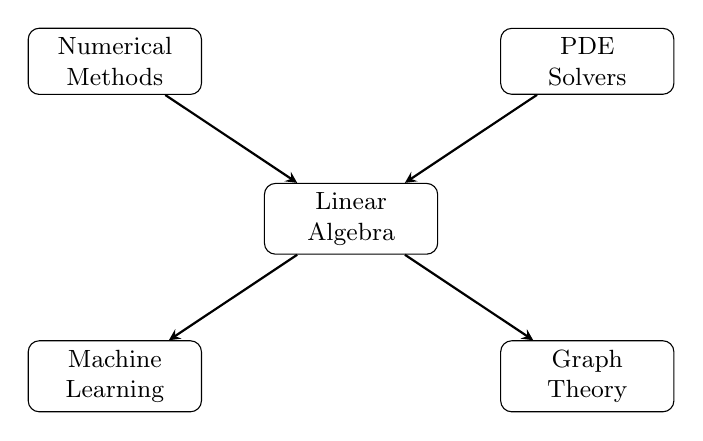
\begin{tikzpicture}[
    concept/.style={rectangle, draw, rounded corners, minimum width=2.2cm,
                    minimum height=0.7cm, align=center, font=\small},
    link/.style={->, thick, >=stealth}
]
    \node[concept] (la) at (0,0) {Linear\\Algebra};
    \node[concept] (num) at (-3,2) {Numerical\\Methods};
    \node[concept] (pde) at (3,2) {PDE\\Solvers};
    \node[concept] (ml) at (-3,-2) {Machine\\Learning};
    \node[concept] (graph) at (3,-2) {Graph\\Theory};

    \draw[link] (num) -- (la);
    \draw[link] (pde) -- (la);
    \draw[link] (la) -- (ml);
    \draw[link] (la) -- (graph);
\end{tikzpicture}
\caption{Concept map connecting core topics.}
\label{fig:concept-map}
\end{figure}

\subsection{Data Flow for an Iterative Solver}

\begin{figure}[htbp]
\centering
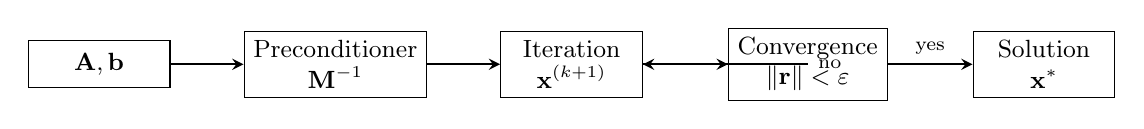
\begin{tikzpicture}[
    box/.style={rectangle, draw, minimum width=1.8cm, minimum height=0.6cm,
                align=center, font=\small},
    arr/.style={->, thick, >=stealth}
]
    \node[box] (input) at (0,0) {$\mathbf{A}, \mathbf{b}$};
    \node[box] (precond) at (3,0) {Preconditioner\\$\mathbf{M}^{-1}$};
    \node[box] (iterate) at (6,0) {Iteration\\$\mathbf{x}^{(k+1)}$};
    \node[box] (check) at (9,0) {Convergence\\$\|\mathbf{r}\| < \varepsilon$};
    \node[box] (output) at (12,0) {Solution\\$\mathbf{x}^*$};

    \draw[arr] (input) -- (precond);
    \draw[arr] (precond) -- (iterate);
    \draw[arr] (iterate) -- (check);
    \draw[arr] (check) -- node[above, font=\scriptsize]{yes} (output);
    \draw[arr] (check) |- node[right, font=\scriptsize, pos=0.2]{no} (iterate);
\end{tikzpicture}
\caption{Data flow of a preconditioned iterative solver.}
\label{fig:dataflow}
\end{figure}

\subsection{Sparse Matrix Structure}

\begin{figure}[htbp]
\centering
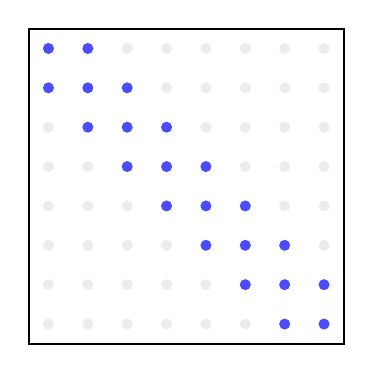
\begin{tikzpicture}[scale=0.5]
    \foreach \i in {1,...,8} {
        \foreach \j in {1,...,8} {
            \pgfmathparse{abs(\i-\j) <= 1 ? 1 : 0}
            \pgfmathtruncatemacro{\val}{\pgfmathresult}
            \ifnum\val=1
                \fill[blue!70] (\j,-\i) circle (4pt);
            \else
                \fill[gray!15] (\j,-\i) circle (4pt);
            \fi
        }
    }
    \draw[thick] (0.5,-0.5) rectangle (8.5,-8.5);
\end{tikzpicture}
\caption{Sparsity pattern of a tridiagonal matrix ($n=8$). Nonzeros shown in blue.}
\label{fig:sparsity}
\end{figure}

% ------------------------------------------------------------
\section{pgfplots: Performance Comparison}

\begin{figure}[htbp]
\centering
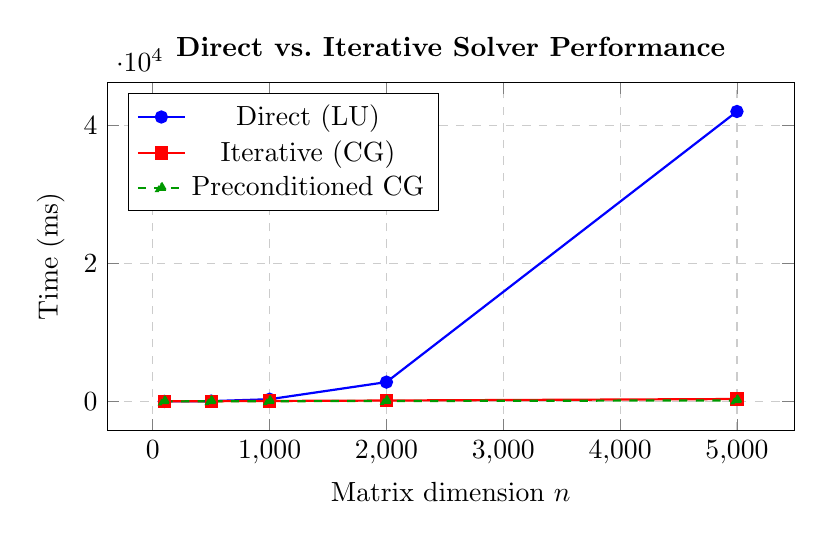
\begin{tikzpicture}
\begin{axis}[
    width=0.85\textwidth,
    height=6cm,
    xlabel={Matrix dimension $n$},
    ylabel={Time (ms)},
    legend pos=north west,
    grid=major,
    grid style={dashed, gray!40},
    title={\textbf{Direct vs.\ Iterative Solver Performance}},
]
    \addplot[blue, thick, mark=*] coordinates {
        (100, 2) (500, 45) (1000, 320) (2000, 2800) (5000, 42000)
    };
    \addlegendentry{Direct (LU)}

    \addplot[red, thick, mark=square*] coordinates {
        (100, 8) (500, 35) (1000, 65) (2000, 130) (5000, 350)
    };
    \addlegendentry{Iterative (CG)}

    \addplot[green!60!black, thick, mark=triangle*, dashed] coordinates {
        (100, 5) (500, 18) (1000, 32) (2000, 60) (5000, 150)
    };
    \addlegendentry{Preconditioned CG}
\end{axis}
\end{tikzpicture}
\caption{Scaling: $O(n^3)$ direct solvers vs.\ near-linear iterative methods.}
\label{fig:perf-comparison}
\end{figure}

\begin{figure}[htbp]
\centering
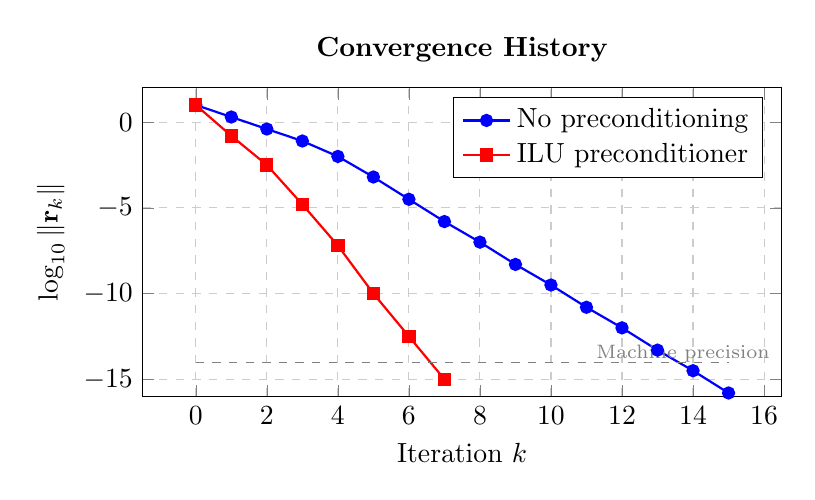
\begin{tikzpicture}
\begin{axis}[
    width=0.8\textwidth,
    height=5.5cm,
    xlabel={Iteration $k$},
    ylabel={$\log_{10}\|\mathbf{r}_k\|$},
    legend pos=north east,
    grid=major,
    grid style={dashed, gray!40},
    title={\textbf{Convergence History}},
    ymin=-16, ymax=2,
]
    \addplot[blue, thick, mark=*] coordinates {
        (0, 1) (1, 0.3) (2, -0.4) (3, -1.1) (4, -2.0) (5, -3.2)
        (6, -4.5) (7, -5.8) (8, -7.0) (9, -8.3) (10, -9.5)
        (11, -10.8) (12, -12.0) (13, -13.3) (14, -14.5) (15, -15.8)
    };
    \addlegendentry{No preconditioning}

    \addplot[red, thick, mark=square*] coordinates {
        (0, 1) (1, -0.8) (2, -2.5) (3, -4.8) (4, -7.2) (5, -10.0)
        (6, -12.5) (7, -15.0)
    };
    \addlegendentry{ILU preconditioner}

    \addplot[dashed, gray] coordinates {(0, -14) (15, -14)};
    \node[anchor=west, font=\scriptsize, gray] at (axis cs: 11, -13.5)
        {Machine precision};
\end{axis}
\end{tikzpicture}
\caption{Residual convergence for a SPD system ($n = 2000$). ILU preconditioning
reaches machine precision in fewer iterations.}
\label{fig:convergence}
\end{figure}

% ------------------------------------------------------------
\section{Python Implementation}

\begin{listing}[htbp]
\centering
\begin{minted}{python}
import numpy as np
from scipy.sparse import diags
from scipy.sparse.linalg import spsolve, cg

def solve_tridiagonal(n: int) -> dict:
    """Solve a tridiagonal SPD system using direct and iterative methods."""
    diagonals = [
        -np.ones(n - 1),   # sub-diagonal
         4 * np.ones(n),   # main diagonal
        -np.ones(n - 1),   # super-diagonal
    ]
    T = diags(diagonals, offsets=[-1, 0, 1], format="csr")

    rng = np.random.default_rng(42)
    b = rng.standard_normal(n)

    x_direct = spsolve(T, b)
    x_iter, info = cg(T, b, tol=1e-12, maxiter=500)

    return {
        "direct_error": np.linalg.norm(T @ x_direct - b),
        "iterative_error": np.linalg.norm(T @ x_iter - b),
        "converged": info == 0,
    }

if __name__ == "__main__":
    results = solve_tridiagonal(n=5000)
    print(f"Direct residual:    {results['direct_error']:.2e}")
    print(f"Iterative residual: {results['iterative_error']:.2e}")
    print(f"Converged:          {results['converged']}")
\end{minted}
\caption{Tridiagonal solver using SciPy's sparse linear algebra.}
\label{lst:solver}
\end{listing}

% ============================================================
%  CHAPTER 3
% ============================================================
\chapter{Applications and Exercises}

\section*{Learning Objectives}
\begin{enumerate}[label=\textbf{LO\arabic*.}, leftmargin=3em]
    \item Apply matrix factorisations to least-squares problems.
    \item Use the SVD to analyse ill-conditioned systems.
    \item Solve graded exercises demonstrating mastery of the material.
\end{enumerate}

% ------------------------------------------------------------
\section{Singular Value Decomposition}

\begin{theorem}[SVD Existence]\label{thm:svd}
Every $\mathbf{A} \in \mathbb{R}^{m \times n}$ admits a decomposition
$\mathbf{A} = \mathbf{U}\boldsymbol{\Sigma}\mathbf{V}^{\top}$ with
orthogonal $\mathbf{U}$, $\mathbf{V}$ and diagonal $\boldsymbol{\Sigma}$
containing singular values $\sigma_1 \geq \cdots \geq \sigma_p \geq 0$.
\end{theorem}

\begin{example}[Low-Rank Approximation]
For a $100 \times 100$ matrix with $\sigma_k = 1/k$, truncating the SVD at
rank $r = 10$ gives $\|\mathbf{A} - \mathbf{A}_r\|_F \approx 0.31$, the
best rank-$r$ approximation by the Eckart--Young theorem.
\end{example}

% ------------------------------------------------------------
\section{Least-Squares via the Normal Equations}

The least-squares problem $\argmin_{\mathbf{x}} \|\mathbf{Ax} -
\mathbf{b}\|_2$ has the normal equations solution
$\mathbf{A}^{\top}\mathbf{A}\,\mathbf{x} = \mathbf{A}^{\top}\mathbf{b}$.

\begin{theorem}[Normal Equations Condition]\label{thm:normal-eq}
If $\mathbf{A}$ has full column rank, then $\mathbf{A}^{\top}\mathbf{A}$ is
SPD with $\kappa_2(\mathbf{A}^{\top}\mathbf{A}) = \kappa_2(\mathbf{A})^2$.
\end{theorem}

\begin{proof}
Since $\mathbf{A}$ has full column rank, $\mathbf{A}^{\top}\mathbf{A}$ is SPD.
The eigenvalues satisfy $\lambda_i(\mathbf{A}^{\top}\mathbf{A}) =
\sigma_i(\mathbf{A})^2$, so $\kappa_2(\mathbf{A}^{\top}\mathbf{A}) =
\sigma_1^2 / \sigma_n^2 = \kappa_2(\mathbf{A})^2$.
\end{proof}

\begin{remark}
Forming $\mathbf{A}^{\top}\mathbf{A}$ squares the condition number.
Use QR or SVD for ill-conditioned problems.
\end{remark}

% ------------------------------------------------------------
\section{Key Terms}

\begin{description}[style=nextline, leftmargin=3em]
    \item[Condition Number]
        Sensitivity of a linear system to perturbations. $\kappa = 10^k$
        means roughly $k$ digits of accuracy are lost.
    \item[LU Factorisation]
        $\mathbf{A} = \mathbf{LU}$ decomposition enabling efficient solution
        of multiple right-hand sides.
    \item[Sparse Matrix]
        Most entries are zero; stored in CSR, CSC, or COO formats.
    \item[Preconditioner]
        Matrix $\mathbf{M} \approx \mathbf{A}^{-1}$ accelerating iterative
        solver convergence.
    \item[Singular Value Decomposition]
        $\mathbf{A} = \mathbf{U}\boldsymbol{\Sigma}\mathbf{V}^{\top}$
        revealing rank, range, and numerical structure.
    \item[Schur Complement]
        $\mathbf{S} = \mathbf{A}_{22} -
        \mathbf{A}_{21}\mathbf{A}_{11}^{-1}\mathbf{A}_{12}$; central to
        domain decomposition.
    \item[Strict Diagonal Dominance]
        $|a_{ii}| > \sum_{j \neq i} |a_{ij}|$; implies nonsingularity and
        Jacobi/Gauss--Seidel convergence.
    \item[Conjugate Gradient]
        Optimal Krylov method for SPD systems minimising the $\mathbf{A}$-norm
        of the error at each step.
\end{description}

% ------------------------------------------------------------
\section{Exercises}

\subsection*{Level~$\star$}

\begin{enumerate}[label=\textbf{\thesection.\arabic*}]
    \item Compute the LU factorisation of
    $\mathbf{A} = \begin{pmatrix} 3 & 1 \\ 6 & 4 \end{pmatrix}$
    by hand. Verify that $\mathbf{PA} = \mathbf{LU}$.
    \label{ex:lu-hand}

    \item Show that $\kappa(\mathbf{I}_n) = 1$ for any induced norm.
    \label{ex:cond-id}

    \item Write out the first three Jacobi iterations for the system in
    \autoref{ex:3x3}, starting from $\mathbf{x}^{(0)} = \mathbf{0}$.
    \label{ex:jacobi-manual}
\end{enumerate}

\subsection*{Level~$\star\star$}

\begin{enumerate}[resume, label=\textbf{\thesection.\arabic*}]
    \item Prove that if $\mathbf{A}$ is SPD, the Cholesky factorisation
    $\mathbf{A} = \mathbf{LL}^{\top}$ exists and is unique.
    \label{ex:cholesky}

    \item Derive the residual bound
    $\|\mathbf{b} - \mathbf{Ax}_k\| \leq
    \|\mathbf{T}_J\|^k \|\mathbf{b} - \mathbf{Ax}_0\|$
    for the Jacobi method.
    \label{ex:residual}

    \item Using \autoref{lst:solver}, implement a 2D Laplacian solver and
    plot convergence history with \textsc{pgfplots}.
    \label{ex:laplacian}
\end{enumerate}

\subsection*{Level~$\star\star\star$}

\begin{enumerate}[resume, label=\textbf{\thesection.\arabic*}]
    \item Let $\mathbf{A}$ be tridiagonal Toeplitz with diagonal $2$ and
    off-diagonals $-1$. Prove $\rho(\mathbf{T}_J) = \cos(\pi/(n+1))$.
    \label{ex:jacobi-spectral}

    \item Design a parallel preconditioner for block-partitioned systems.
    Analyse convergence theoretically and validate on $n = 10{,}000$.
    \label{ex:parallel-precond}

    \item Derive BiCGSTAB from first principles, prove its short-recurrence
    property, and compare against GMRES on a convection--diffusion problem.
    \label{ex:bicgstab}
\end{enumerate}

% ============================================================
%  BIBLIOGRAPHY
% ============================================================
\printbibliography[heading=subbibintoc, title=References]

\end{document}
